\documentclass[12pt,a4paper]{article}
\usepackage{personal-mathphys}

% Additional package for sample plots
\usepackage{pgfplots}
\pgfplotsset{compat=1.18}

\begin{document}

% Creating a professional title page using our custom command
\maketitlepage{Quantum Harmonic Oscillator:\\A Mathematical Analysis}{Alice Johnson}{Department of Mathematical Physics\\University of Science}{\today}

\maketocpage

\newpage

\section{Introduction}

The quantum harmonic oscillator serves as a fundamental model in quantum mechanics, providing insights into systems ranging from vibrating molecules to quantum field theory. In this document, we'll explore its mathematical foundation and physical implications.

\section{Mathematical Framework}

Let's begin by establishing the key mathematical concepts. The time-independent Schrödinger equation for the quantum harmonic oscillator is given by:

\begin{equation}
    -\frac{\planck^2}{2m}\frac{d^2\psi}{dx^2} + \frac{1}{2}kx^2\psi = E\psi
\end{equation}

\begin{theorem}{Energy Spectrum}{spectrum}
The energy levels of a quantum harmonic oscillator are quantized according to:
\[ E_n = \planck\omega(n + \frac{1}{2}), \quad n = 0,1,2,\ldots \]
where $\omega = \sqrt{k/m}$ is the angular frequency.
\end{theorem}

\begin{definition}{Ground State}{ground}
The ground state wavefunction of the quantum harmonic oscillator is:
\[ \psi_0(x) = \left(\frac{m\omega}{\pi\planck}\right)^{1/4} 
    e^{-\frac{m\omega x^2}{2\planck}} \]
This represents the state of lowest possible energy, $E_0 = \frac{1}{2}\planck\omega$.
\end{definition}

\section{Physical Interpretations}

\begin{law}{Zero-Point Energy}{zpe}
A quantum harmonic oscillator cannot have zero energy, even at absolute zero temperature. The minimum energy is:
\[ E_0 = \frac{1}{2}\planck\omega \]
This is a direct consequence of the Heisenberg Uncertainty Principle.
\end{law}

\begin{experiment}{Energy Level Observation}{observation}
Using laser spectroscopy, we can observe transitions between energy levels. The energy difference between adjacent levels is constant:
\[ \Delta E = E_{n+1} - E_n = \planck\omega \]
This leads to equally spaced spectral lines in absorption and emission spectra.
\end{experiment}

\section{Mathematical Analysis}

Consider the raising and lowering operators:

\begin{align}
    \hat{a} &= \sqrt{\frac{m\omega}{2\planck}}\left(x + \frac{i}{m\omega}\hat{p}\right) \\
    \hat{a}^\dagger &= \sqrt{\frac{m\omega}{2\planck}}\left(x - \frac{i}{m\omega}\hat{p}\right)
\end{align}

\begin{lemma}{Commutation Relation}{commutation}
The commutator of the raising and lowering operators is:
\[ [\hat{a}, \hat{a}^\dagger] = 1 \]
This relation is fundamental to the algebraic solution of the quantum harmonic oscillator.
\end{lemma}

\begin{note}{Quantum Numbers}{quantum}
The quantum number $n$ determines not only the energy but also the shape of the wavefunction. Higher $n$ values correspond to more nodes in the wavefunction.
\end{note}

\section{Visualization}

Let's visualize the probability densities for the first few energy states:

\begin{center}
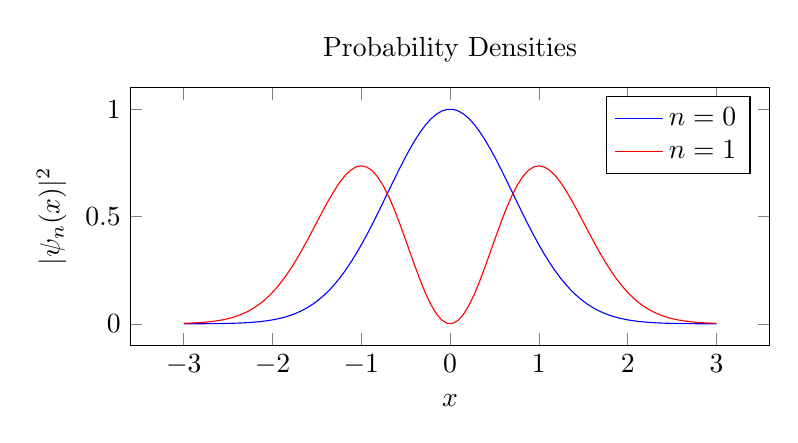
\begin{tikzpicture}
\begin{axis}[
    xlabel=$x$,
    ylabel=$|\psi_n(x)|^2$,
    title={Probability Densities},
    legend pos=north east,
    width=0.8\textwidth,
    height=0.4\textwidth
]
\addplot[blue, domain=-3:3, samples=100] {exp(-x^2)}; % n=0
\addplot[red, domain=-3:3, samples=100] {2*x^2*exp(-x^2)}; % n=1
\legend{$n=0$,$n=1$}
\end{axis}
\end{tikzpicture}
\end{center}

\section{Applications}

The quantum harmonic oscillator model applies to various physical systems:

\begin{itemize}
    \item Molecular vibrations in diatomic molecules
    \item Phonons in crystalline solids
    \item Quantum optics and laser physics
\end{itemize}

\begin{definition}{Coherent States}{coherent}
Coherent states are the quantum states that most closely resemble classical harmonic oscillator behavior. They are eigenstates of the annihilation operator:
\[ \hat{a}|\alpha\rangle = \alpha|\alpha\rangle \]
where $\alpha$ is a complex number.
\end{definition}

\bibliography{references}
\end{document}
